%\documentclass[a4paper,10pt]{article}
\documentclass[tikz, margin = 5mm]{standalone}
\usepackage[utf8]{inputenc}

\usepackage{tikz}
\usetikzlibrary{shapes.geometric, arrows}

\tikzstyle{startstop} = [rectangle, rounded corners, minimum width=3cm, minimum height=1cm,text centered, draw=black, fill=red!30]
\tikzstyle{process} = [rectangle, minimum width=3cm, minimum height=1cm, text centered, draw=black, fill=orange!30]
\tikzstyle{decision} = [diamond, minimum width=3cm, minimum height=1cm, text centered, draw=black, fill=green!30]
\tikzstyle{arrow} = [thick,->,>=stealth]

%opening
\title{}
\author{}

\begin{document}

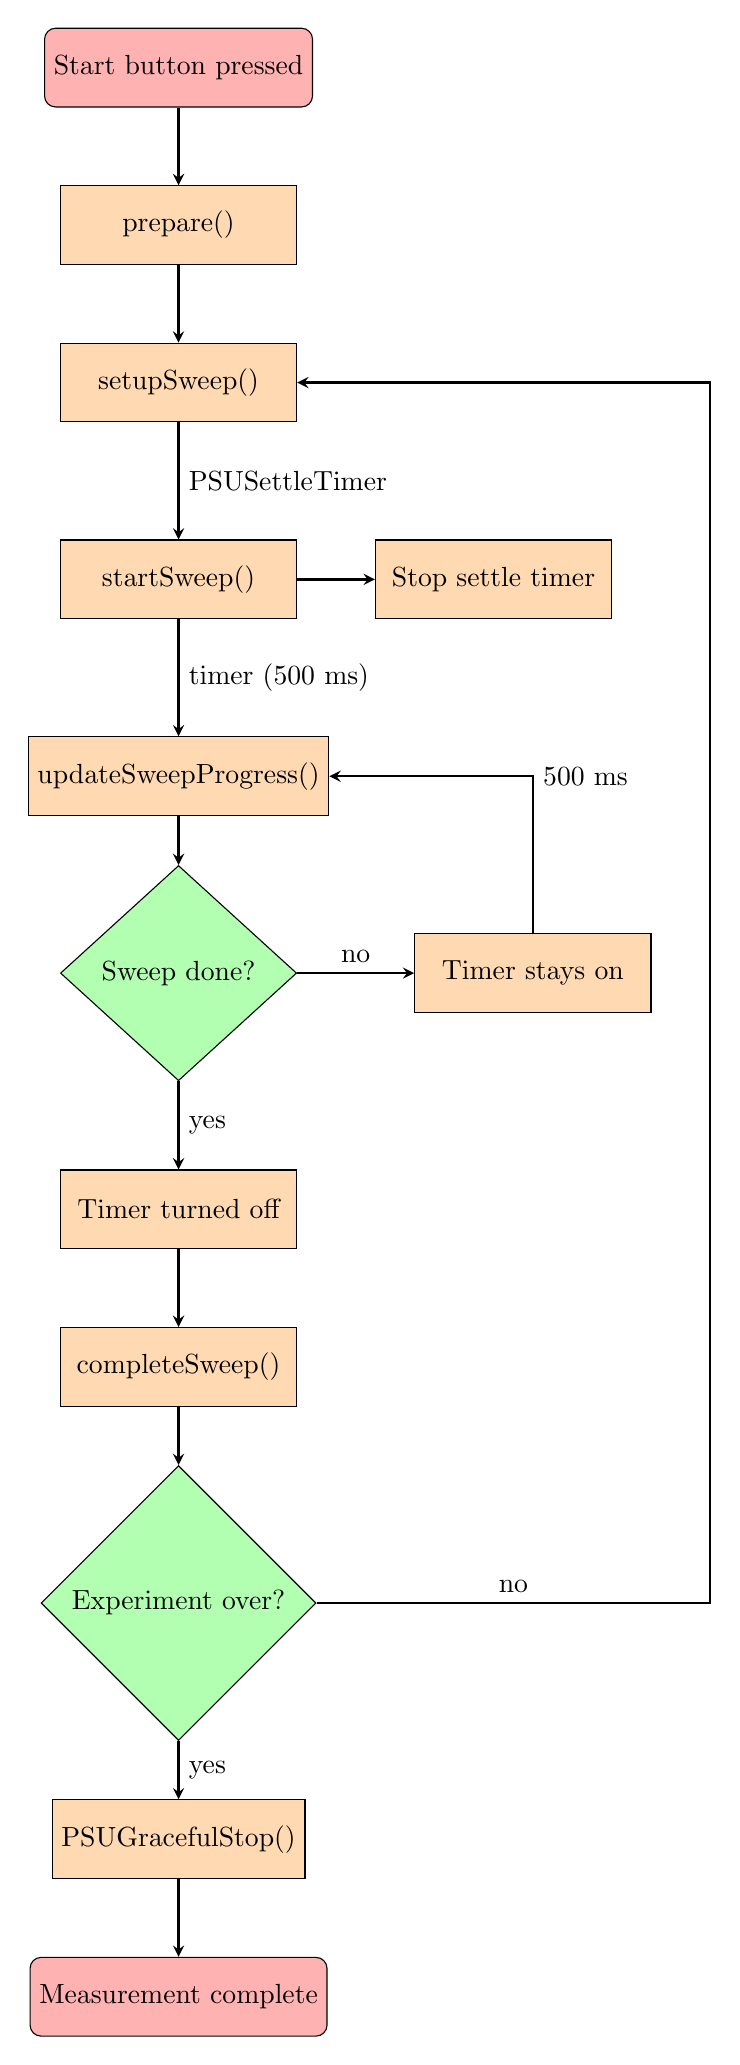
\begin{tikzpicture}[node distance=2cm]
    \node (start) [startstop] {Start button pressed};
    \node (prepare) [process, below of=start] {prepare()};
    \node (setupsweep) [process, below of=prepare] {setupSweep()};
    \node (startsweep) [process, below of=setupsweep, yshift = -0.5cm] {startSweep()};
    \node (settletimeroff) [process, right of=startsweep, xshift = 2cm] {Stop settle timer};
    \node (updatesweepprogress) [process, below of=startsweep, yshift = -0.5cm] {updateSweepProgress()};
    \node (sweepdone) [decision, below of=updatesweepprogress, yshift = -0.5cm] {Sweep done?};
    \node (sweeptimeron) [process, right of = sweepdone, xshift = 2.5cm] {Timer stays on};
    \node (sweeptimeroff) [process, below of = sweepdone, yshift = -1cm] {Timer turned off};
    \node (completesweep) [process, below of=sweeptimeroff] {completeSweep()};
    \node (expdone) [decision, below of=completesweep, yshift = -1cm] {Experiment over?};
    \node (psuoff) [process, below of = expdone, yshift = -1cm] {PSUGracefulStop()};
    \node (stop) [startstop, below of = psuoff] {Measurement complete};

    \draw [arrow] (start) -- (prepare);
    \draw [arrow] (prepare) -- (setupsweep);
    \draw [arrow] (setupsweep) -- node[anchor=west] {PSUSettleTimer} (startsweep);
    \draw [arrow] (startsweep) -- (settletimeroff);
    \draw [arrow] (startsweep) -- node[anchor = west] {timer (500 ms)} (updatesweepprogress);
    \draw [arrow] (updatesweepprogress) -- (sweepdone);
    \draw [arrow] (sweepdone) -- node [anchor = south] {no} (sweeptimeron);
    \draw [arrow] (sweeptimeron) |- node[anchor=west] {500 ms} (updatesweepprogress);
    \draw [arrow] (sweepdone) -- node [anchor = west] {yes} (sweeptimeroff);
    \draw [arrow] (sweeptimeroff) -- (completesweep);
    \draw [arrow] (completesweep) -- (expdone);
    \draw [arrow] (expdone) -- node [anchor = west] {yes} (psuoff);
    \draw [arrow] (psuoff) -- (stop);
    \draw [arrow] (expdone.east) -- node[anchor = south] {no} ++(5,0) |- (setupsweep.east);

\end{tikzpicture}


\end{document}
